\documentclass[a4paper,12pt]{report}

\usepackage{url}
\usepackage{graphicx}
\usepackage[utf8]{inputenc}
\usepackage{float}
\usepackage{hyperref}

% Questo commentalo se vuoi scrivere in inglese.
\usepackage[italian]{babel}

\usepackage[italian]{cleveref}

\title{I coloni di Cesena}

\author{Bartoli Davide && Guerrini Alex && Ronchi Mattia && Samor\`i Andrea}
\date{\today}


\begin{document}

\maketitle

\tableofcontents

\chapter{Analisi}

\section{Requisiti}

Il software mira alla realizzazione di una versione virtuale del gioco da tavolo \href{https://it.wikipedia.org/wiki/I_coloni_di_Catan}{I coloni di Catan}. Il gioco simula la colonizzazione di un'isola contesa da più giocatori, che tentano di accumulare risorse e ostacolare gli avversari. L'isola è costituita da un insieme di celle esagonali, ciascuna corrispondente ad un tipo di risorsa (lana, legno, grano, minerali, argilla) ed avente un numero da 2 a 12. Ciascun giocatore possiede delle proprietà, che gli permettono di guadagnare le risorse ad essa circostanti. Oltre alle proprietà sono presenti delle strade, che permettono al giocatore di espandere il proprio dominio e collegare eventuali proprietà già possedute. Ogni proprietà o strada necessita, per la sua costruzione, di specifiche risorse.

\subsection{Requisiti funzionali}
\begin{itemize}
    \item La generazione della mappa di gioco avviene in modo casuale seguendo alcune regole.
    \item Il videogioco dovrà consentire di partecipare a 4 giocatori in una modalità a turni. Ciascun turno consiste nel lancio di una coppia di dadi, la cui somma determina quali celle producono la propria risorsa, che viene guadagnata dal giocatore se possiede una proprietà ad essa adiacente. Nel caso la somma sia 7, il giocatore di turno deve posizionare il \textit{Brigante}, una speciale pedina, in una cella, bloccandone la produzione di risorse
    \item Il giocatore di turno può effettuare le seguenti azioni:
    \begin{itemize}
        \item proporre scambi di risorse agli altri giocatori
        \item costruire proprietà/strade
        \item acquistare carte sviluppo
    \end{itemize}
    \item Il software dovrà occuparsi di calcolare i punteggi di ogni giocatore, determinati dalle proprietà possedute, al fine di determinare il vincitore della partita.
\end{itemize}

\subsection{Requisiti non funzionali}
\begin{itemize}
    \item Il sistema deve essere efficiente nell'utilizzo delle risorse hardware e reattivo alle azioni dei giocatori
    \item L'interfaccia di gioco deve essere minimale, semplice e intuitiva
\end{itemize}

\section{Analisi e modello del dominio}

L'entità principale del sistema è il \textit{game manager}, che coordina la gestione degli aspetti principali del gioco: mappa, turni, proprietà, risorse e scambi. Il game manager dovrà poter accedere alla mappa, contenente le proprietà dei vari giocatori, e mantenerne aggiornato lo stato. Tali proprietà prendono il nome di strade, colonie e città. Ciascuna proprietà necessita, per la sua costruzione, di un certo numero di risorse. Il game manager dovrà gestire la corretta associazione di ciascuna proprietà o risorsa al corrispettivo giocatore. Infine, il game manager dovrà poter relazionarsi con i giocatori e la mappa per ottenere le informazioni necessarie a realizzare ciò che è descritto sopra.\\
Per quanto riguarda gli aspetti impegnativi, si ritiene la mappa e le adiacenze tra caselle,strade e proprietà un aspetto ostico in quanto le caselle sono di forma esagonale

\begin{figure}[H]
\centering{}
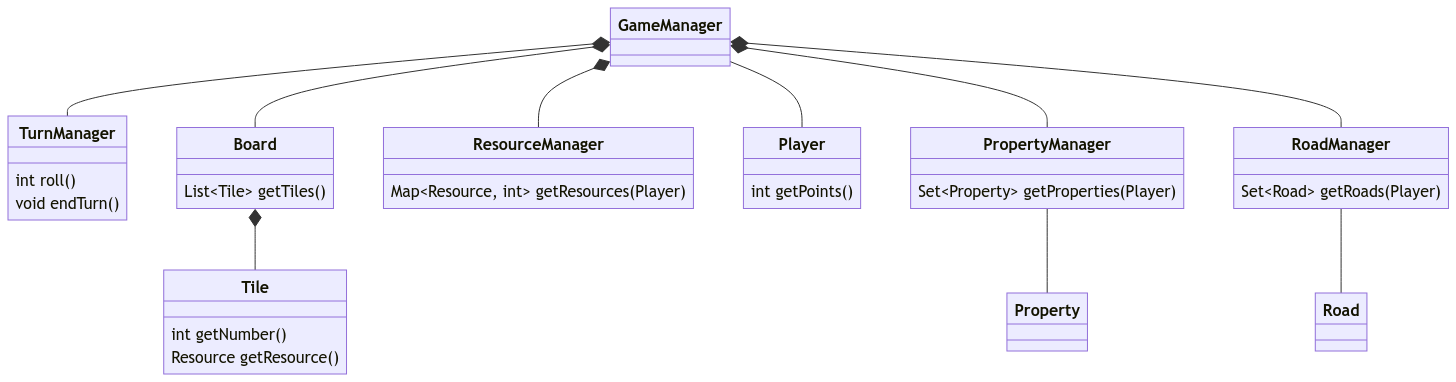
\includegraphics[scale=0.3]{imgs/analysis.png}
\caption{Schema UML dell'analisi del problema, con rappresentate le entità principali ed i rapporti fra loro}
\label{img:analysis}
\end{figure}

\chapter{Design}

\section{Architettura}

L'architettura del software utilizza il pattern MVC. I componenti principali sono:
\begin{itemize}
    \item AppView
    \item MainController
    \item GameManager
\end{itemize}
AppView reagisce agli input forniti dall'utente e notifica il controller, che si occupa eventualmente di chiamare il model per aggiornare lo stato interno. Il controller si occupa anche di notificare la view di reagire a un cambiamento e aggiornarsi di conseguenza. MainController è suddiviso in ulteriori controller più specifici in base alle classi del model coinvolte.\\
Con questa architettura, sostituire la view è semplice in quanto è sufficiente che implementi l'interfaccia AppView, composta da pochi metodi necessari al controller per mantenerla aggiornata.

\begin{figure}[H]
\centering{}
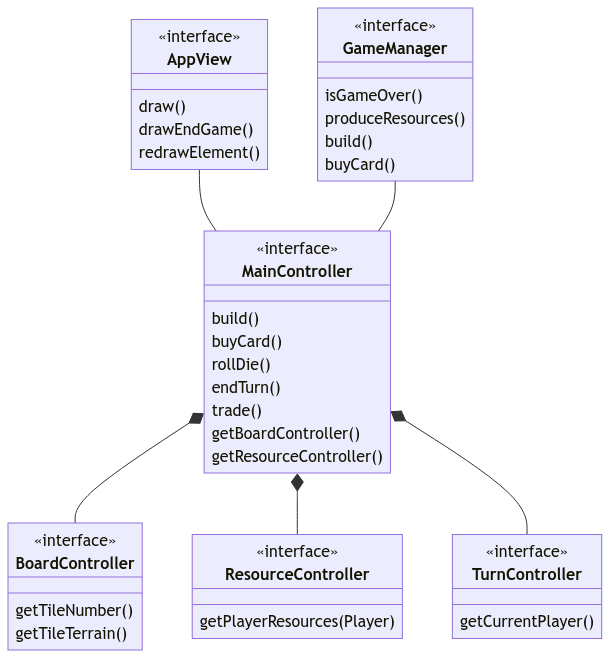
\includegraphics[scale=0.6]{imgs/design.png}
\caption{Schema UML dell'analisi del problema, con rappresentate le entità principali ed i rapporti fra loro}
\label{img:analysis}
\end{figure}

\section{Design dettagliato}
\subsection{Bartoli Davide}
\paragraph{Problema:} Gestione della posizione delle caselle e dei strade e proprietà. Questo è reso complesso dal fatto che le caselle hanno forma esagonale.
\paragraph{Soluzione:} Ho realizzato le interfacce TilePosition, RoadPosition e PropertyPosition. Le caselle vengono indicizzate tramite la loro riga e la loro colonna, e le righe di indice dispari sono traslate verso destra di mezzo esagono. RoadPosition e PropertyPosition invece sono composte di una TilePosition e una delle 6 possibili direzioni (una RoadPosition di fatto indica uno dei 6 lati dell'esagono mentre una PropertyPosition uno dei 6 vertici). Notare che questa rappresentazione di RoadPosition e PropertyPosition non è univoca dato che ad esempio una strada può essere vista dai due esagoni che tocca, per questo ho realizzato il metodo equals per tenerne conto, utilizzando metodi che calcola le altre posizioni equivalenti. 

\begin{figure}[H]
\centering{}
\includegraphics[scale=0.6]{imgs/board.png}
\caption{Posizioni delle caselle}
\label{img:analysis}
\end{figure}
\begin{figure}[H]
\centering{}
\includegraphics[scale=0.45]{imgs/positions.png}
\label{img:analysis}
\end{figure}
\paragraph{Problema:} Gestione della mappa di gioco.
\paragraph{Soluzione:} Ho creato la classe BoardImpl, che implementa l'interfaccia Board, che salva tutte le caselle in una mappa da TilePosition a Tile. L'interfaccia Tile permette di ottenere informazioni come il numero e il tipo di terreno di quella casella.
\begin{figure}[H]
\centering{}
\includegraphics[scale=0.35]{imgs/BoardImpl.png}
\label{img:analysis}
\end{figure}

\paragraph{Problema:} Aggiornare la view della mappa
\paragraph{Soluzione:} Ho creato le classi PropertyView, RoadView e TileView che estendono classi di JavaFX e implementano il metodo draw() per ridisegnarsi. In questo modo posso chiamare draw solamente sulle parti necessarie in modo da non dover rigenerare ogni volta tutta la view.
\begin{figure}[H]
\centering{}
\includegraphics[scale=0.35]{imgs/boardView.png}
\label{img:analysis}
\end{figure}
\subsection{Guerrini Alex}
La mia parte del progetto consisteva nel lavorare sulla gestione dei turni di gioco, la gestione delle carte sviluppo e la creazione dei menu di gioco per la corretta inizializzazione della partita.
\paragraph{Problema:}Sistema che tenga traccia del turno corrente e delle azioni che possono svolgere i giocatori in base al turno in cui si trovano.
\paragraph{Soluzione:}Ho progettato un'interfaccia \textit{TurnManager} che definisce i metodi necessari per il conteggio dei turni per alleggerire il lavoro del \textit{GameManager}, come il recupero del giocatore corrente, la fine del turno e il lancio dei dadi. Successivamente, ho implementato questa interfaccia nella classe \textit{TurnManagerImpl}, che gestisce la logica dei turni e delle operazioni ad essi associate.
 All'interno del \textit{GameManager} è presente la logica finale che utilizza sia il turn manager che altri componenti creati dai miei compagni per poter determinare le azioni dei giocatori in base al ciclo di turni corrente.
\paragraph{Problema:}Corretta gestione dei turni e divisione in cicli dei turni di gioco per rispettare le regole del gioco "Coloni di Catan".
\paragraph{Soluzione:}Utilizzo del pattern Iterator in \textit{TurnManager}.
\paragraph{Utilizzo di design pattern:}Nella progettazione è stato utilizzato il pattern Iterator per gestire in modo efficiente il ciclo dei turni. L'iteratore generato è stato implementato in modo da garantire un ciclo di turni che attraversa tutti i giocatori nell'ordine corretto con un corretto reverse dell'ordine nel secondo ciclo di turni.
\begin{figure}[H]
\centering{}
\includegraphics[scale=0.4]{imgs/GameManagerTurnManager.png}
\caption{Schema UML del TurnManager e del GameManager}
\label{img:analysis}
\end{figure}
\paragraph{Problema:}Creazione e gestione del mazzo delle carte sviluppo
\paragraph{Soluzione:}Ho progettato un'interfaccia \textit{DevelopmentCards} che definisce i metodi necessari per la gestione delle carte sviluppo, come la pesca di una carta dal mazzo e la verifica se il mazzo è vuoto. Successivamente, ho implementato concretamente questa interfaccia nella classe \textit{DevelopmentCardsImpl}, che gestisce il mazzo di carte sviluppo e fornisce i metodi per pescare carte e verificare lo stato del mazzo.
\paragraph{Problema:}Gestione della pescata delle carte sviluppo e dei loro effetti sul giocatore.
\paragraph{Soluzione:}Ho creato i tipi di carte sviluppo attraverso \textit{CardType.java}, ne ho gestito la pescata che comprende la spesa delle risorse dei giocatori per pescare e l'effetto di queste carte sul giocatore attraverso \textit{buyCard} all'interno di \textit{GameManager}.
\begin{figure}[H]
\centering{}
\includegraphics[scale=0.4]{imgs/GameManagerDevelopmentCards.png}
\caption{Schema UML del TurnManager e delle DevelopmentCards}
\label{img:analysis}
\end{figure}
\subsection{Ronchi Mattia}
\paragraph{Problema} Struttura della mappa di gioco variabile.
\paragraph{Soluzione} La mappa di gioco viene creata utilizzando il pattern Strategy: la classe GameMapGenerator è la classe che rappresenta la strategia, mentre BeginnerGameMapGenerator e RandomGameMapGenerator sono le sue due implementazioni.
\begin{figure}[H]
\centering{}
\includegraphics[scale=0.4]{imgs/gameMapGenerator.png}
\caption{Schema UML della generazione della mappa}
\label{img:analysis}
\end{figure}
\paragraph{Problema} Personalizzazione delle impostazioni
\paragraph{Soluzione} Ho utilizzato una interfaccia GameSettings, che viene utilizzata da GameManager per modificare l'inizializzazione di alcuni componenti. Attualmente esiste una sola implementazione di questa interfaccia, GameSettingsJSON (che recupera le impostazioni tramite un file JSON con uno schema predefinito) ma è semplice crearne altre varianti.
\begin{figure}[H]
\centering{}
\includegraphics[scale=0.4]{imgs/gameSettings.png}
\caption{Schema UML della gestione del punteggio}
\label{img:analysis}
\end{figure}
\paragraph{Problema} Gestione dei punteggi
\paragraph{Soluzione} Essendo i punti vittoria ottenibili attraverso diverse tipologie di azioni, ho scelto di delegare ai singoli gestori delle entità (RoadManager e PropertyManager) la loro gestione (fatta eccezione per le carte sviluppo, in quanto quest'ultime, a differenza di altre entità, non hanno un proprietario ma vengono utilizzate e subito scartate). I singoli gestori gestiscono il punteggio direttamente all'interno dei metodi corrispondenti alle azioni che comportano una modifica del punteggio (questo è reso possibile dal fatto che essi non hanno bisogno di accedere, per gestire i punteggi, ad altro che le entità da loro gestite).\\
Un'altra valida alternativa sarebbe stata quella di gestire i punteggi all'interno di GameManager (ad esempio tramite una classe interna). In questo caso si ha il vantaggio di poter disattivare a piacimento alcuni fattori che modificano il punteggio (es. bonus della strada più lunga) ma al prezzo di appesantire la classe. Al limite, si potrebbe anche decidere di delegare l'intera gestione dei punti a un gestore separato (PointsManager).
\begin{figure}[H]
\centering{}
\includegraphics[scale=0.4]{imgs/gameManagerPoints.png}
\caption{Schema UML della gestione del punteggio}
\label{img:analysis}
\end{figure}
\subsection{Samor\'i Andrea}
Nella parte da me effettuata, ho cercato di ideare il codice per agevolare il pi\`u possibile il riuso e l'estendibilit\`a. Un esempio \`e nelle risorse, dove basta inserire nell'enum dedicato (ResourceType) la nuova risorsa, e il programma continuer\`a funzioner\`a alla perfezione.
\paragraph{Problema:}  gestione delle propriet\`a dei vari giocatori.
\paragraph{Soluzione:} ho deciso di utilizzare un \textit{Property Manager} per gestire le propriet\`a in gioco piuttosto che assegnare nella classe \textit{Player} i metodi e le strutture dati per le propriet\`a. Questo \`e stato fatto per non appesantire gli altri componenti.
\paragraph{Problema:} gestione delle risorse dei vari elementi del gioco (giocatori e mappa).
\paragraph{Soluzione:} ho deciso di utilizzare un \textit{Resource Manager} per gestire le risorse in gioco piuttosto che assegnare nelle varie classi (Player e Bank) i metodi e le strutture dati per le risorse. Questo \`e stato fatto per non appesantire gli altri componenti.
\paragraph{Problema:}effettuare operazioni di scambio di risorse sia con altri giocatori sia con la banca.

\paragraph{Soluzione:}ho risolto creando una interfaccia \textit{ResourceOwner} che viene implementata sia dalla classe Player che dalla classe Bank. All'interno del ResourceManager  ogni operazione di modifica e scambio delle risorse prende come input un ResourceOwner, cos\`i da permettere le sopracitate operazioni sia tra due giocatori che tra giocatore e banca. Quando lo richiedono, metodi del \textit{ResourceManager}     
\begin{figure}[H]
\centering{}
\includegraphics[scale=0.4]{imgs/resourceManager.png}
\caption{Schema UML del Resource manager}
\label{img:analysis}
\end{figure}
\paragraph{Problema:} mandare a schermo messaggi di diversa natura, in base a ci\`o che accade nel gioco.
\paragraph{Soluzione:} ho utilizzato il pattern \textit{Factory}, creando una \textit{MessageFactory} che crea vari messaggi in base a ci\`o che \`e richiesto. Questo permette, in caso si vogliano creare nuovi messaggi da inviare a schermo, di aggiungere semplicemente altri metodi create alla fabbrica.
\begin{figure}[H]
\centering{}
\includegraphics[scale=0.4]{imgs/messageFactory.png}
\caption{Schema UML del Resource manager}
\label{img:analysis}
\end{figure}
\paragraph{Problema:} creazione di elementi simili nella view. Infatti, serve creare l'immagine delle varie risorse con vari elementi affianco.
\paragraph{Soluzione:} Per evitare di riscrivere inutilmente codice, ho creato una ResourceViewFactory, che permette di creare differenti tipi di visuale della risorsa in base alla necessit\`a.

\chapter{Sviluppo}
\section{Testing automatizzato}
Si è deciso di sottoporre a test automatizzato tramite JUnit alcune funzionalità dei componenti principali:
\begin{itemize}
    \item RoadPosition,PropertyPosition: funzioni che verificano l'adiacenza tra strade/proprietà/caselle
    \item GameManager: funzioni che simulano i primi turni di gioco e la produzione di risorse
    \item RoadManager: funzioni che verificano la costruzione di strade e la meccanica della strada più lunga
    \item ResourceManager: funzioni che verificano la gestione delle risorse e degli scambi
    \item TurnManager: funzioni che verificano la gestione dei turni
    \item Player: funzioni che verificano l'aggiornamento dei punti
    \item GameMapGenerator: funzioni che verificano la generazione di una mappa di gioco aderente alle regole
\end{itemize}


\section{Note di sviluppo}
\subsection{Bartoli Davide}
\subsubsection{Utilizzo di Stream e lambda expressions}
Usati in numerosi punti. Ad esempio \url{https://github.com/davi-bart/OOP23-coloni-ces/blob/dfbfa6f4eb46f9ed826c6d568074ce085e25fd25/src/main/java/it/unibo/controller/impl/MainControllerImpl.java#L112C9-L115C46}
\subsubsection{Utilizzo della libreria Apache Commons}
Ad esempio \url{https://github.com/davi-bart/OOP23-coloni-ces/blob/0950c43bdd3aee77487a8cbdb0aed8111b5f7916/src/main/java/it/unibo/common/TileCoordinatesImpl.java#L7C5-L7C54}
\subsubsection{Utilizzo della libreria JavaFX}
Utilizzata in tutto il progetto. Un esempio \`e \url{https://github.com/davi-bart/OOP23-coloni-ces/blob/bb5e6b1ecf814446af912da8460983d4d5c8e953/src/main/java/it/unibo/view/PropertyView.java#L56C1-L61C1}
\subsubsection{Utilizzo dei record}
Ad esempio \url{https://github.com/davi-bart/OOP23-coloni-ces/blob/88e2af616a6af9e8dcd04c7efb93fcd7eb89262b/src/main/java/it/unibo/view/MessageView.java#L3C1-L3C69}
\subsubsection{Utilizzo di Optional}
Ad esempio \url{https://github.com/davi-bart/OOP23-coloni-ces/blob/7b6d50c738ca08d9b8f1d0930366eff178d45141/src/main/java/it/unibo/model/property/PropertyManagerImpl.java#L58C5-L58C28}

\subsection{Guerrini Alex}
\subsubsection{Utilizzo di Stream e lambda expressions}
Utilizzato in tutto il progetto. Un esempio \`e \url{https://github.com/davi-bart/OOP23-coloni-ces/blob/94d6e93730b0de4e9a41878b0cd8de7cdda4f1f1/src/main/java/it/unibo/model/turn/TurnManagerImpl.java#L37C1-L46C81}
\subsubsection{Utilizzo della libreria JavaFX}
Un esempio \`e \url{https://github.com/davi-bart/OOP23-coloni-ces/blob/94d6e93730b0de4e9a41878b0cd8de7cdda4f1f1/src/main/java/it/unibo/view/app/StartMenuView.java#L138C1-L148C33}
\subsection{Ronchi Mattia}
\subsubsection{Utilizzo della libreria}
Permalink: \url{https://github.com/davi-bart/OOP23-coloni-ces/blob/2759276c233b2d366192f17430bb8f9c7de6f275/src/main/java/it/unibo/model/mapgenerator/RandomGameMapGenerator.java#L83}
\subsubsection{Utilizzo della libreria JGraphT}
Utilizzato in RoadManagerImpl per il calcolo della strada più lunga: \url{https://github.com/davi-bart/OOP23-coloni-ces/blob/fac3379ddae2ca7015850973811087d3b8f247bd/src/main/java/it/unibo/model/road/RoadManagerImpl.java#L59}
\subsubsection{Utilizzo della libreria Jackson}
Utilizzata per la lettura del file JSON: \url{https://github.com/davi-bart/OOP23-coloni-ces/blob/fac3379ddae2ca7015850973811087d3b8f247bd/src/main/java/it/unibo/model/GameSettingsJSON.java#L50}
\subsubsection{Utilizzo di Optional}
Ad esempio \url{https://github.com/davi-bart/OOP23-coloni-ces/blob/fac3379ddae2ca7015850973811087d3b8f247bd/src/main/java/it/unibo/model/road/RoadManagerImpl.java#L89}
\subsubsection{Utilizzo di Stream}
Utilizzate massivamente. Un esempio è \url{https://github.com/davi-bart/OOP23-coloni-ces/blob/2759276c233b2d366192f17430bb8f9c7de6f275/src/main/java/it/unibo/model/GameManagerImpl.java#L269}
\subsubsection{Utilizzo di method reference}
Ad esempio \url{https://github.com/davi-bart/OOP23-coloni-ces/blob/fac3379ddae2ca7015850973811087d3b8f247bd/src/main/java/it/unibo/model/road/RoadManagerImpl.java#L79}

\subsection{Samor\'i Andrea}
\subsubsection{Utilizzo della libreria JavaFX}
Utilizzata in tutto il progetto. Un esempio \`e \url{https://github.com/davi-bart/OOP23-coloni-ces/blob/94d6e93730b0de4e9a41878b0cd8de7cdda4f1f1/src/main/java/it/unibo/view/resource/ResourcesViewFactory.java#L37C8-L41C47}
\subsubsection{Utilizzo di \texttt{Stream} e lambda expressions}
Uso massivo. Il seguente \`e un esempio:\url{https://github.com/davi-bart/OOP23-coloni-ces/blob/94d6e93730b0de4e9a41878b0cd8de7cdda4f1f1/src/main/java/it/unibo/model/resource/ResourceManagerImpl.java#L32-L33}
Propongo anche una pozione di codice dove viene utilizzata anche la method reference: \url{https://github.com/davi-bart/OOP23-coloni-ces/blob/bf20339e5603deddb49259c841ca6f19fb6432c5/src/main/java/it/unibo/model/resource/ResourceManagerImpl.java#L131}
\subsubsection{Utilizzo di Optional}
Permalink:\url{https://github.com/davi-bart/OOP23-coloni-ces/blob/94d6e93730b0de4e9a41878b0cd8de7cdda4f1f1/src/main/java/it/unibo/model/property/PropertyManagerImpl.java#L33-L34}

\chapter{Commenti finali}
\section{Bartoli Davide}
Il mio ruolo è stato rivolto principalmente alla rappresentazione della mappa nel model e nella view.
Nella parte da me prodotta penso che uno dei punti di forza siano le rappresentazioni delle posizioni degli oggetti, che penso abbiano astratto in maniera efficace la rappresentazione sottostante e siano state facili da utilizzare anche dai miei compagni di gruppo. 
Uno dei punti deboli è stato il design della BoardView. Infatti, anche a causa della difficoltà iniziale con JavaFX, è stato necessario modificarlo numerose volte. Inoltre avevo creato una versione iniziale della BoardView prima di aver definito fino in fondo la struttura del model, e questo ha necessitato cambiamenti successivi, anche se sono soddisfatto del risultato finale.
In generale mi ritengo soddisfatto del risultato raggiunto dal gruppo.
\section{Guerrini Alex}
Il mio ruolo all'interno del gruppo era quello di gestire i turni di gioco e ciò che ne conseguiva, gestire i menu di gioco e gestire la lista delle carte sviluppo e la loro logica.
I principali punti deboli che ho riscontrato sono: un'iniziale difficoltà nel comprendere appieno le funzionalità più avanzate di Java, l'utilizzo di Git per la gestione del progetto e l'uso di JavaFX per l'implementazione dell'interfaccia grafica. Tuttavia, ho fatto uno sforzo cosciente nel partecipare ad un gruppo di studenti molto competenti, con l'intento di imparare da loro e migliorare le mie abilità, questo ha fatto in modo che io faticassi inizialmente a stare al passo ma ha anche fatto in modo che imparassi molte cose e molto più in fretta rispetto a quanto avrei appreso in un altro gruppo.
I miei punti di forza riscontrati in questo progetto sono:
Per quanto riguarda il codice  ho cercato di utilizzare nomi di variabili e metodi esplicativi, migliorando così la leggibilità e la comprensione del codice da parte degli altri membri del gruppo limitando a zero le incomprensioni e inoltre ho adottato una struttura ben organizzata, dividendo le funzionalità in moduli distinti e garantendo una separazione facilmente comprensibile delle responsabilità rendendo più semplice la modifica e l'estensione del codice più avanti nel progetto.
Mentre per quanto riguarda i punti di forza riscontrati non inerenti al codice ho avuto una buona capacità di adattamento ad una situazione a me sconosciuta cioè il lavoro di programmazione in gruppo.
Principali difficolt\`a riscontrate durante il progetto:
\begin{itemize}
    \item Quantità di lavoro necessario: ho sottovalutato la mole di lavoro necessaria al completamento del progetto, questo è stato causato da una mia inesperienza nella programmazione di un progetto di gruppo.
    \item Uso di Git: Inizialmente ho riscontrato difficoltà nell'uso di Git e la risoluzione di possibili merge conflict. La sua complessità iniziale ha richiesto tempo per essere compresa e utilizzata in modo corretto.
    \item Uso di JavaFX: JavaFX è una libreria con cui non ero familiare e che non avevo approfondito dopo l'unica lezione di laboratorio in cui è stata spiegata.
\end{itemize}
\section{Ronchi Mattia}
Il mio ruolo all'interno del gruppo è stato rivolto principalmente nella parte controller e model e penso di aver avuto un impatto rilevante nella progettazione dell'architettura generale. A tal proposito, ho proposto nella parte iniziale del progetto una architettura che infine si è rilevata problematica e ha costretto tutto il gruppo a spostare diverse parti di codice da un punto all'altro (mantenendone però invariata la logica), comportando una rilevante perdita di tempo.\\
In generale, ritengo di aver svolto nel complesso un buon lavoro (in base alle capacità che ritengo di avere). Tra i punti di forza farei rientrare l'aver realizzato un codice per quanto possibile semplice, chiaro e ben documentato. Per quanto riguarda i punti di debolezza, oltre al problema sopracitato, aggiungerei anche l'aver sottovalutato la quantità del carico di lavoro necessario alla realizzazione del progetto.
\section{Samor\'i Andrea}
Nella parte da me prodotta, i punti di debolezza da me riscontrati sono la iniziale parziale ignoranza di alcune delle funzionalit\`a pi\`u avanzate del linguaggio, che ho cercato di colmare andando avanti con il progetto e mettendo in pratica ci\`o che abbiamo visto a lezione. Infatti credo che mettere in pratica e confrontarsi giornalmente con altri studenti (sicuramente pi\`u competenti di me) siano le principali cause del mio miglioramento.\\
I punti di forza nella parte da me prodotta sono la semplicit\`a nel comprendere cosa deve fare ogni singolo componente. Questo ho cercato di effettuarlo utilizzando nomi "parlanti", che possano dare una idea effettiva di ci\`o che la parte di codice deve fare.\\
A livello di progetto, sono abbastanza soddisfatto del risultato del lavoro del gruppo. Abbiamo cercato di organizzare e dividerci il codice il meglio possibile e di dividerci in maniera equa la mole di lavoro (forse in questo caso non riuscendoci al meglio). \\
Le principali difficolt\`a da me riscontrate durante il progetto sono:
\begin{itemize}
    \item Utilizzo di JavaFX: una libreria nuova, che non avevo visto a lezione (essendo stato assente durante la presentazione). Cercare per alcuni componenti se si poteva fare ci\`o che volevo non \`e stato banale, soprattutto perch\`e gli esempi di codice effettivo nella documentazione sono scarsi.
    \item Utilizzo di Git: soprattutto inizialmente, non avendolo mai usato se non in questo corso, ho trovato difficile utilizzare Git in modo proficuo.
    \item Ammontare di lavoro: inizialmente avevo sottovalutato l'ammontare di lavoro, e quindi mi sono ritrovato un po' spiazzato quando ho capito che ci\`o che avevo previsto fosse una sotto-stima della realt\`a.
    \item Organizzare il lavoro in un progetto: essendo la mia prima esperienza in un progetto relativamente grande, ho trovato difficile (soprattutto nelle fasi iniziali) organizzare e analizzare l'interezza del progetto, e non pensare solo alle singole entit\`a, ma anche ai rapporti che ci devono essere tra esse.
\end{itemize}
\section{Difficoltà incontrate e commenti per i docenti}

\appendix
\chapter{Guida utente}
All'avvio dell'applicazione, viene presentata una schermata in cui viene presentata un'area in cui inserire i nomi dei giocatori (al massimo 4) e un pulsante per iniziare il gioco. Il gioco si svolge a turni ed ogni turno è svolto come segue:
\begin{enumerate}
    \item lancio del dado
    \item assegnazione delle risorse prodotte
    \item il giocatore, a questo punto, può decidere di svolgere una delle seguenti azioni:
    \begin{itemize}
        \item costruire una strada, una colonia o una città
        \item acquistare una carta sviluppo
        \item effettuare scambi con altri giocatori o con la banca
        \item terminare il turno
    \end{itemize}
\end{enumerate}
Per costruire è sufficiente cliccare la mappa nel punto desiderato.

\chapter{Regole del gioco}
\begin{itemize}
    \item durante i suoi primi 2 turni, ogni giocatore deve costruire una colonia e una strada
    \item per ogni turno di un ciclo successivo al secondo, va lanciato una coppia di dadi. Tutti i giocatori che possiedono una proprietà vicina ad una casella avente come numero la somma dei dadi lanciati, ricevono la risorsa prodotta dal terreno di quella casella (1 risorsa se la proprietà è una colonia, 2 risorse se la proprietà è una città)
    \item una strada può essere posizionata solamente vicino ad una proprietà posseduta dal giocatore o ad un'altra strada
    \item una proprietà può essere posizionata solamente su una strada posseduta dal giocatore (ad eccezione dei primi 2 turni) e se ad almeno 2 strade di distanza da tutte le altre proprietà
    \item se il numero estratto è 7, tutti i giocatori con più di 7 risorse devono scartarne la metà
    \item è possibile scambiare con la banca offrendo 4 risorse dello stesso tipo in cambio di 1 qualsiasi altra risorsa
    \item il giocatore che ha la strada più lunga (almeno 5 strade) ottiene 2 punti bonus
\end{itemize}

\end{document}